\documentclass{article}

\usepackage{enumitem}
\usepackage{amsmath}
\usepackage{amsfonts}
\usepackage{amssymb}
\usepackage{textcomp}
\usepackage{gensymb}
\usepackage[dvipsnames]{xcolor}
\usepackage[margin=0.5in]{geometry}
\usepackage[hidelinks,bookmarks=false]{hyperref}

\usepackage{environ}
\NewEnviron{centerframebox}{\begin{center}\fbox{\parbox{0.92\textwidth}{\BODY}}\end{center}}

\let\oldphi\phi
\let\phi\varphi
\newcommand{\Z}{\mathbb{Z}}

\hypersetup{
  colorlinks=true,
  urlcolor=MidnightBlue,
  linkcolor=WildStrawberry,
  % pdfborderstyle={/S/U/W 2}
}

\title{Cryptography \\ Exercise Sheet 8}
\author{
  AAAAAAAAAA AAAAAAA \\
  \href{mailto:AAAAAAAAAAAAAAAAAAAA}{AAAAAAAAAAAAAAAAAAAA}
}

\usepackage{graphicx}
\graphicspath{ {.} {./img/} }

\usepackage[listings,many]{tcolorbox}
\makeatletter
\newtcblisting{mylisting}{
  listing only,
  breakable, enhanced jigsaw,
  listing engine=listings,
  colback=gray!20,
  listing options={
    language=python,
    keywordstyle=\color{blue},
    basicstyle=\ttfamily,
    stringstyle=\color{ForestGreen},
    commentstyle=\color{gray},
    ndkeywordstyle={\color{orange}},
    identifierstyle=\color{black},
    numbers=none,
    showstringspaces=false,
    aboveskip={0\p@ \@plus 6\p@}, belowskip={0\p@ \@plus 6\p@},
    columns=fullflexible, keepspaces=true,
    breaklines=true, breakatwhitespace=true,
    extendedchars=false,
    inputencoding=utf8,
    upquote=true,
    xleftmargin=-25pt,
  }
}
\makeatother

\begin{document}
  \maketitle

  \setcounter{section}{8}
  \subsection{Chinese Remainder Theorem}
  \begin{centerframebox}
    Use the Chinese Remainder Theorem to compute a number $x \in \Z$, $0 \leq x < 210$ such that
    \[ x \operatorname{rem} 7 = 1, \qquad x \operatorname{rem} 15 = 3, \qquad x \operatorname{rem} 2 = 0. \]
  \end{centerframebox}
  To solve a system of equations using the Chinese Remainder Theorem we need to compute the inverses in each base,
  and then the solution can be derived by the following sum:
  \[ x = \sum_{i=1}^n r_i M_i M_i^{-1} \mod M \]
  Where $M = \prod_{i=1}^n m_i = m_1 \cdot m_2 \cdot m_3 = 7 \cdot 15 \cdot 2 = 210$, $M_i = \prod_{j != i} m_j$
  and $M_i^{-1}$ is calculated in $\Z_{m_i}$.
  \[
    \begin{array}{c|c|c|c|c|c}
      i & r_i & m_i & M_i & M_i^{-1} & r_i M_i M_i^{-1} \\
      \hline
      1 & 1 & 7 & 30 & 4 & 120 \\
      2 & 3 & 15 & 14 & 14 & 588 \\
      3 & 0 & 2 & 105 & 1 & 0 \\
    \end{array}
  \]
  The sum turns out to be $x = 120+588 = 78 \pmod{210}$. We can check that it satisfies all the initial equations.

  \subsubsection{All integers}
  \begin{centerframebox}
    Give the set of all integers $x$ solving the previous system of congruences and explain why the previous task had to have a solution.
  \end{centerframebox}
  The previous task had to have a solution, because $7$, $15$ and $2$ are coprime.
  The is stated directly by the Chinese Remainder Theorem.
  The theorem also states that all solutions have the same remainder for $M$,
  i.e. $N_1 \equiv N_2 \pmod{M}$ where $N_1$ and $N_2$ are two solutions.

  So the solution set for $\Z$ will be $S = \{k \in \Z : 78 + k \cdot 210\}$.

  \subsection{Compositeness Testing}
  \begin{centerframebox}
    In this exercise we put hands on the compositeness tests discussed in the lecture.
  \end{centerframebox}
  \subsubsection{Miller Rabin test}
  \begin{centerframebox}
    Implement the loop body of the Miller Rabin test in a programming
    language of your choice with input $N$ and $a$, rather than picking $a$
    randomly.
  \end{centerframebox}
  \begin{mylisting}
    def miller_rabin_body(n, a):
      s, d = 0, n - 1
      while d % 2 == 0:
        s, d = s + 1, d // 2
      # `s` is the number of times we could divide n-1 by 2

      x = pow(a, d, n)
      if x == 1 or x == n - 1:
        return "maybe prime"

      for _ in range(1, s):
        x = (x * x) % n
        if x == 1:
          return "not prime"
        if x == n - 1:
          return "maybe prime"

      return "not prime"
  \end{mylisting}
  \subsubsection{Fermat test}
  \begin{centerframebox}
    Implement the loop body of the Fermat test in a programming language of your choice, i.e. take the loop body of the Miller Rabin test
    and omit the step testing for non-trivial square roots of $1$.
  \end{centerframebox}
  \begin{mylisting}
    def fermat_test(n, a):
      x = pow(a, n-1, n)
      if x == 1 or x == n-1:
        return "maybe prime"
      else:
        return "not prime"
  \end{mylisting}

  \subsubsection{Run it!}
  \begin{centerframebox}
    Now, let's run it! Execute the Miller Rabin test with
    \begin{enumerate}
      \item[(iii)] $N = 41,\, a = 2$
      \item[(iv)] $N = 57,\, a = 37$
      \item[(v)] $N = 1105,\, a = 47$
      \item[(vi)] $N = 1105,\, a = 2$
    \end{enumerate}
  \end{centerframebox}
  \begin{mylisting}
    # (iii) N = 41, a = 2    -> maybe prime
    print((41, 2), miller_rabin_body(41, 2))
    # (iv) N = 57, a = 37    -> not prime
    print((57, 37), miller_rabin_body(57, 37))
    # (v) N = 1105, a = 47   -> maybe prime
    print((1105, 47), miller_rabin_body(1105, 47))
    # (vi) N = 1105, a = 2   -> not prime
    print((1105, 2), miller_rabin_body(1105, 2))
  \end{mylisting}
  We got the correct result for all but $N = 1105,\, a = 47$ example.
  $1105$ is obviously divisible by $5$, so it is not prime.
  But this is expected!

  \subsubsection{Fermat liars}
  \begin{centerframebox}
    Compute the number of Fermat liars for $N = 35$, i.e. the number of
    choices $a \in \Z^\times_N$ for which the Fermat test returns $N$ ``maybe prime''.
  \end{centerframebox}
  \begin{mylisting}
    # (vii) Compute the number of Fermat liars for N = 35  -> 4  [1, 6, 29, 34]
    # [1, 34] are trivial
    print("Fermat liars for N = 35:", [i for i in range(35) if fermat_test(35, i) == "maybe prime"])
  \end{mylisting}
  We got 4 liars and 2 of them are trivial $1$ and $N-1$ values, which always lie!

  \subsubsection{Miller Rabin liars}
  \begin{centerframebox}
    Compute the number of Miller Rabin liars for $N = 35$, i.e. the number of
    choices $a \in \Z^\times_N$ for which the Miller Rabin test returns $N$ ``maybe prime''.
  \end{centerframebox}
  \begin{mylisting}
    # (vii) Compute the number of Miller Rabin liars for N = 35  -> 2  [1, 34]
    # both trivial
    print("Miller Rabin liars for N = 35:", [i for i in range(35) if miller_rabin_body(35, i) == "maybe prime"])
  \end{mylisting}
  We got only the trivial liars! This is the best result we can hope for.

  \subsubsection{More liars}
  \begin{centerframebox}
    Do the same for $N = 561$.
  \end{centerframebox}
  \begin{mylisting}
    # (ix) Do the same for N = 561  -> 10  [1, 50, 101, 103, 256, 305, 458, 460, 511, 560]
    print("Miller Rabin liars for N = 561:", [i for i in range(561) if miller_rabin_body(561, i) == "maybe prime"])
  \end{mylisting}
  Now we get a lot of liars. As expected.

  \subsection{Pseudo compositeness test}
  \begin{centerframebox}
    The strong pseudo primality test decomposes $N - 1 = 2^r s$ with $s$ odd and chooses a random $a \in \Z_N$,
    and computes $a^s,\, a^{2s},\, \dots,\, a^{2^r s}$.
    It answers ``$N$ is not prime'' if this sequence does not contain $1$ or, if that the first $1$ is not
    in the first position then the preceding number is not $-1$. Otherwise, it answers ``$N$ may be prime''.
  \end{centerframebox}
  This is just the Miller Rabin test with only one iteration.

  \subsubsection{Which properties of primes are used?}
  We use Fermat's Theorem, i.e. the property that every element in $\Z_n$ is invertible if and only if $n$ is a prime.

  \subsubsection{Probability}
  \begin{centerframebox}
    Why didn't we tell the test to answer ``$N$ is prime'' in the second
    case? (Give an estimate for the probability that the test detects that a
    given composite number $N$ is not prime.)
  \end{centerframebox}
  Because Miller Rabin liars exist.
  The probability can be estimated based on the Miller Rabin test.
  It has an upper bound for the error probability of $1/4^k$.
  So with $k=1$, the probability is just $1/4$.

  \subsection{Carmichael numbers \& order}
  TODO

  \subsection{Prime number theorem}
  \begin{centerframebox}
    Use some programming system, eg. Sage, to generate a plot of the following functions to learn a bit about the prime counting function $\pi$ over the ranges $1..100$ and $1..1000$.
  \end{centerframebox}
  \begin{mylisting}
    # naive primality test
    # it's fine to use it here, because all the numbers are under 1000
    def is_prime(n):
      if n < 2:
        return False
      i = 2
      while i*i <= n:
        if n % i == 0:
          return False
        i += 1
      return True

    def prime_pi(n):
      return sum(is_prime(i) for i in range(n+1))

    # needed for the Li() logarithmic integral function
    from mpmath import mp
  \end{mylisting}
  We have to use a deterministic primality test, to get guaranteed correct values for $\pi()$.

  \subsubsection{Consider $\pi(x)/\frac{x}{\ln x}$}
  \begin{mylisting}
    import numpy as np
    import matplotlib.pyplot as plt

    def pi_plot_log(n):
      X = np.arange(1, n)
      Y = np.array([prime_pi(i) for i in X])/(X/np.log(X))

      plt.plot(X, Y, label=r"$\pi(x)/\frac{x}{\ln x}$")
      plt.legend()
      plt.show()

    pi_plot_log(100)
    pi_plot_log(1000)
  \end{mylisting}

  \noindent
  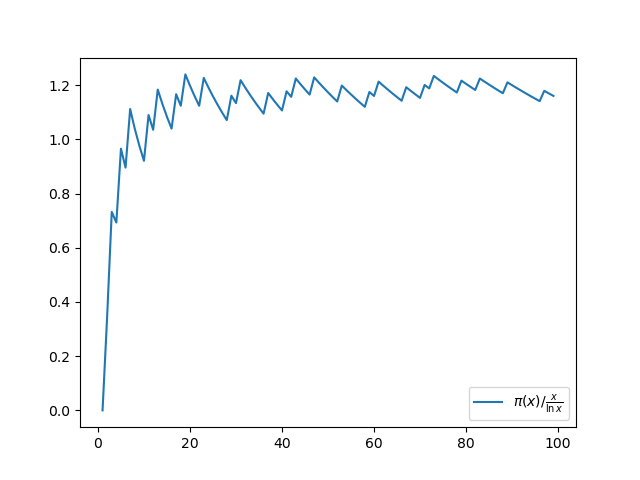
\includegraphics[width=0.5\textwidth]{div100}%
  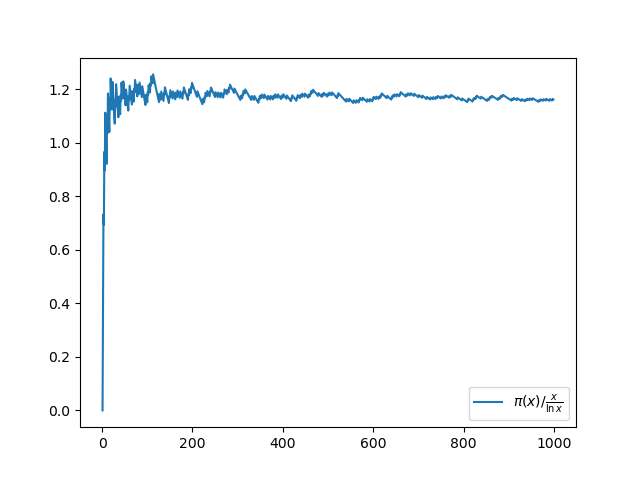
\includegraphics[width=0.5\textwidth]{div1000}

  Looks like it approaches $1.163$.

  \subsubsection{Upper and lower bounds}
  \begin{centerframebox}
    Draw in single plot the three functions in the prime number theorem,
    namely an upper and a lower bound and $\pi$ You may choose the
    bounds of the Schoenfeld or the Dusart version. Or all in one plot.
  \end{centerframebox}
  \begin{mylisting}
    def pi_plot(n, name=""):
      X = np.arange(1, n)
      LI = [float(mp.li(i)) for i in X] # upper bound
      LOG = X/np.log(X) # lower bound
      PI = [prime_pi(i) for i in X]

      plt.plot(X, PI, label=r"$\pi(x)$")
      plt.plot(X, LI, label=r"Li(x)")
      plt.plot(X, LOG, label=r"$\frac{x}{\ln x}$")
      plt.legend()
      plt.show()

    pi_plot(100)
    pi_plot(1000)
  \end{mylisting}
  The upper bound is $\operatorname{Li}(x)$ and the lower bound is $\frac{x}{\ln x}$.
  People usually use just use the lower bound, because it's so much easier to compute.
  Have any of you even seen this $\operatorname{Li}$ function before..?

  \noindent
  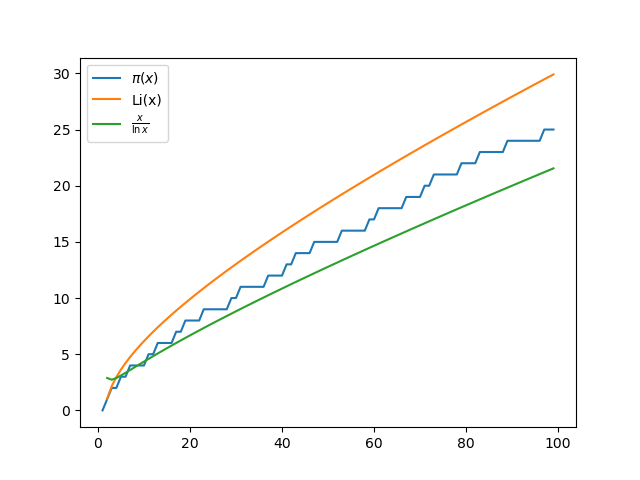
\includegraphics[width=0.5\textwidth]{bounds100}%
  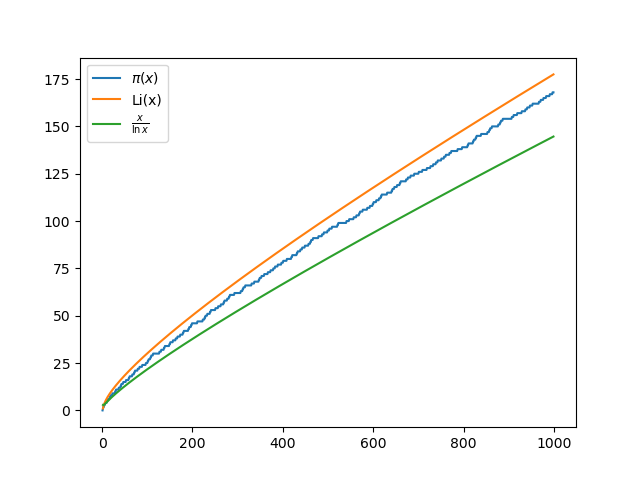
\includegraphics[width=0.5\textwidth]{bounds1000}

  The bounds do, in fact, work.
  If we ignore the small numbers around $\leq 20$.

\end{document}
